\section{Subgrupos, Generadores, Retículos y Grupos cíclicos}

\begin{ejercicio}\label{ej:3.1}
    Describir todos los elementos de los grupos alternados $A_n$, consistentes en las permutaciones pares del $S_n$ correspondiente, para $n = 2$, $n = 3$ y $n = 4$.    
\end{ejercicio}

\begin{ejercicio}\label{ej:3.2}
    Sea $D_n$ el grupo diédrico. Demostrar que el subgrupo de $D_n$ generado por los elementos $\{r^js, r^ks\}$ es todo el grupo $D_n$ siempre que $0 \leq j < k < n$ y $\mcd(k - j, n) = 1$.
\end{ejercicio}

\begin{ejercicio}\label{ej:3.3}
    \begin{enumerate}
        \item Demostrar que el subgrupo de $\SL_2(\bb{Z}_3)$ generado por los elementos
        \[
            i = \begin{pmatrix}
                0 & -1 \\
                1 & 0
            \end{pmatrix}, \quad j = \begin{pmatrix}
                1 & 1 \\
                1 & -1
            \end{pmatrix}
        \]
        es isomorfo al grupo cuaternio $Q_2$.
        \item Demostrar que $\SL_2(\bb{Z}_3)$ y $S_4$ son dos grupos de orden 24 que no son isomorfos.
        \begin{observacion}
            Demostrar que $S_4$ no puede contener a ningún subgrupo isomorfo a $Q_2$.
        \end{observacion}
    \end{enumerate}
\end{ejercicio}

\begin{ejercicio}\label{ej:3.4}
    Razonar que un subconjunto no vacío $X \subseteq G$ de un grupo $G$ es un subgrupo de $G$ si, y sólo si, $X = \langle X \rangle$.
\end{ejercicio}

\begin{ejercicio}\label{ej:3.5}
    Sean $a, b \in G$ dos elementos de un grupo que conmutan entre sí, esto es, para los que $ab = ba$, y de manera que sus órdenes son primos relativos, esto es, $\mcd(O(a), O(b)) = 1$.
    \begin{enumerate}
        \item Razonar que $\langle a \rangle \cap \langle b \rangle = 1$.
        \item Demostrar que $O(ab) = O(a)O(b)$.
    \end{enumerate}
\end{ejercicio}

\begin{ejercicio}\label{ej:3.6}
    Encontrar un grupo $G$ y elementos $a, b \in G$ tales que sus órdenes sean primos relativos, pero para los que no se verifique la igualdad $O(ab) = O(a)O(b)$ del ejercicio anterior.
\end{ejercicio}

\begin{ejercicio}\label{ej:3.7}
    Sea $G$ un grupo y $a, b \in G$ dos elementos de orden finito. ¿Es $ab$ necesariamente de orden finito?
    \begin{observacion}
        Considerar el grupo $\GL_2(\bb{Q})$ y los elementos
        \[
            a = \begin{pmatrix}
                0 & -1 \\
                1 & 0
            \end{pmatrix}, \quad b = \begin{pmatrix}
                0 & 1 \\
                -1 & 1
            \end{pmatrix}.
        \]
    \end{observacion}
\end{ejercicio}

\begin{ejercicio}\label{ej:3.8}
    En el grupo $S_3$ se considera el conjunto
    \[
        H = \{1, (1\ 2\ 3), (1\ 3\ 2)\}.
    \]
    \begin{enumerate}
        \item Demostrar que $H$ es un subgrupo de $S_3$.
        \item Describir las diferentes clases de $S_3$ módulo $H$.
    \end{enumerate}
\end{ejercicio}

\begin{ejercicio}\label{ej:3.9}
    Sea $G$ un grupo finito.
    \begin{enumerate}
        \item Demostrar que si $H \leq G$ es un subgrupo, entonces $[G : H] = |G|$ si, y sólo si, $H = \{1\}$, mientras que $[G : H] = 1$ si, y sólo si, $H = G$.
        \item Demostrar que si se tienen subgrupos $G_2 \leq G_1 \leq G$, entonces
        \[
            [G : G_2] = [G : G_1][G_1 : G_2],
        \]
        \item Demostrar que si se tiene una cadena descendente de subgrupos de la forma
        \[
            G = G_0 \geq G_1 \geq \cdots \geq G_{r - 1} \geq G_r,
        \]
        entonces
        \[
            [G : G_r] = \prod_{i = 0}^{r - 1}[G_i : G_{i + 1}].
        \]
        \item Demostrar que si se tiene una cadena descendente de subgrupos de la forma
        \[
            G = G_0 \geq G_1 \geq \cdots \geq G_{r - 1} \geq G_r = \{1\},
        \]
        entonces
        \[
            |G| = \prod_{i = 0}^{r - 1}[G_i : G_{i + 1}].
        \]
    \end{enumerate}
\end{ejercicio}

\begin{ejercicio}\label{ej:3.10}~
    \begin{enumerate}
        \item Demostrar que si $G$ es un grupo de orden 4, entonces se tiene que o bien $G$ es cíclico, o bien es isomorfo al grupo de Klein.
        \item Demostrar que si $G$ es un grupo de orden 6, entonces se tiene que o bien $G$ es cíclico, o bien es isomorfo al grupo diédrico $D_3$.
    \end{enumerate}
\end{ejercicio}

\begin{ejercicio}\label{ej:3.11}
    Describir los retículos de subgrupos de los siguientes grupos:
    \begin{enumerate}
        \item El grupo $V$ de Klein.
        \item El grupo simétrico $S_3$.
        \item El grupo diédrico $D_4$.
        \item El grupo cuaternio $Q_2$.
        \item El grupo alternado $A_4$.
    \end{enumerate}
\end{ejercicio}

\begin{ejercicio}\label{ej:3.12}
    Fijado un número primo $p$, describe el retículo de subgrupos del grupo cíclico $C_{p^n}$. En particular, describe el retículo de subgrupos del grupo cíclico $C_8$.
\end{ejercicio}

\begin{ejercicio}\label{ej:3.13}
    Demostrar que un grupo finito $G \neq \{1\}$ carece de subgrupos propios, esto es, que su retículo de subgrupos es el de la Figura~\ref{fig:ej13} si, y sólo si, $G = C_p$ es un grupo cíclico de orden primo.
    \begin{figure}
        \centering
        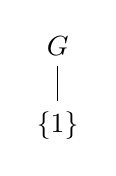
\begin{tikzpicture}[node distance=1cm]
            \node (G)  {$G$};
            \node[below of=G] (1) {$\{1\}$};

            \draw (G) -- (1);
        \end{tikzpicture}
        \caption{Retículo de subgrupos de para el Ejercicio~\ref{ej:3.13}.}
        \label{fig:ej13}
    \end{figure}
\end{ejercicio}

\begin{ejercicio}\label{ej:3.14}
    Describir los retículos de subgrupos de los grupos cíclicos siguentes:
    \begin{enumerate}
        \item $C_6$.
        \item $C_{12}$.
    \end{enumerate}
\end{ejercicio}

\begin{ejercicio}\label{ej:3.15}
    Se considera el grupo cíclico $C_{136}$ de orden 136, con generador $t$. ¿Qué relación hay entre los subgrupos $H_1 = \langle t^{48}, t^{72} \rangle$ y $H_2 = \langle t^{46} \rangle$?
\end{ejercicio}

\begin{ejercicio}\label{ej:3.16}
    Demostrar que el grupo de unidades $\bb{Z}_7^\times$ es un grupo cíclico.
\end{ejercicio}

\begin{ejercicio}\label{ej:3.17}
    Sea $G$ un grupo y sea $C_n$ el grupo cíclico de orden $n$ generado por $x$. Demostrar que:
    \begin{enumerate}
        \item Si $\theta : C_n \to G$ es un homomorfismo de grupos, entonces:
        \begin{equation*}
            O(\theta(x))\mid n, \quad \text{y} \quad \theta(x^k) = \theta(x)^k \quad \forall k \in \{0, \ldots, n - 1\}.
        \end{equation*}

        \item Para cada $g \in G$ tal que $O(g) \mid n$, existe un único homomorfismo de grupos $\theta_g : C_n \to G$ tal que $\theta_g(x) = g$.
        
        \item Si $g \in G$ es tal que $O(g) \mid n$, entonces el morfismo $\theta_g$ es monomorfismo si, y sólo si, $O(g) = n$.
        
        \item Existe un isomorfismo de grupos
        \begin{equation*}
            U(\bb{Z}_n) \cong \Aut(C_n),
        \end{equation*}
        dado por $r \mapsto f_r$ para cada $r = 1, \ldots, n$ con $\mcd(r, n) = 1$, donde el automorfismo $f_r$ se define mediante $f_r(x) = x^r$.

        En particular, $\Aut(C_n)$ es un grupo abeliano de orden $\varphi(n)$.
    \end{enumerate}
\end{ejercicio}

\begin{ejercicio}\label{ej:3.18}~
    \begin{enumerate}
        \item Describir explícitamente el grupo de automorfismos $\Aut(C_8)$.
        \item Demostrar que $\Aut(C_8)$ es isomorfo al grupo de Klein.
    \end{enumerate}
\end{ejercicio}